\documentclass{article}
\usepackage{placeins}
\usepackage{graphicx}
\usepackage{subcaption}
\usepackage{listings}
\usepackage{hyperref}
\usepackage{cleveref}
\usepackage{booktabs, siunitx}
\usepackage{geometry}
\usepackage{minted}
\usepackage{subfiles}
\usepackage{indentfirst}
\usepackage[backend=biber]{biblatex}
\usepackage[svgnames,table]{xcolor}

\addbibresource{ref.bib}
\usemintedstyle{emacs}
\geometry{
 a4paper,
 total={170mm,257mm},
 left=20mm,
 top=20mm,
 }
\graphicspath{ {./images/} }

\title{
Assignment 2 Report\\
\large Fuzzy logic in trading securities
}
\author{Tanat Tangun 630610737}
\date{September 2022}

\begin{document}
\maketitle
This report is about the result of my fuzzy logic implementation on Rust language for 261456 - INTRO COMP INTEL FOR CPE class
assignment. This report will be about how fuzzy logic can help in trading securities and other assets. 
If you are interested to know how I implement the fuzzy logic and use it to help in trading securities and other assets
, you can see the source code on my 
\href{https://github.com/RiwEZ/FuzzyLogicOnRust}{Github repository} or in this document appendix.

\section*{Introduction}
The term ``securities and other assets" in our report include securities such as stock, bonds, currencies, and other assets
i.e. crypto-currency, house price, etc. In this report, we will focus on crypto-currency such as Ethereum. Before we delve 
further, let's understand that we are not trying to create more profit than any other techniques but we are trying to learn how
to create fuzzy logic and explore how it might be useful for trading.

\subsection*{Technical Indicators} 
\label{tech}
According to \cite{technical_indicator}, ``Technical indicators are heuristic or pattern-based signals produced by the price, volume, 
and/or open interest of a security or contract used by traders who follow technical analysis.
By analyzing historical data, technical analysts use indicators to predict future price movements."

We are trying to use technical indicators to help decide when to entry or exit to make a profit trade. Techinal indicators
that we will use are RSI (Relative Strength Index) and Bollinger Bands.

\subsubsection*{RSI - Relative Strength Index}
According to \cite{rsi} ``The relative strength index (RSI) is a momentum indicator used in technical analysis. 
RSI measures the speed and magnitude of a security's recent price changes to evaluate overvalued or 
undervalued conditions in the price of that security."
RSI is a value in range $[0, 100]$ and the value at time $t$ is defined as follows:
$$
    \text{RSI} = 100 - \frac{100}{1 + \text{RS}}
$$
where $\text{RS}$ is the relative strength of the last $n$ sessions and its defined as:
$$
    \text{RS} = \frac{\text{AverageGain}_t(n)}{\text{AverageLoss}_t(n)}
$$
where $\text{AverageGain}_t(n)$ and $\text{AverageLoss}_t(n)$ are the average of the gains ($\text{price}_t > \text{price}_{t-1}$) 
and losses ($\text{price}_t < \text{price}_{t-1}$), obtained in the last n sessions. That is, from time $t - (n - 1)$ to time $t$. 
However, theses values are usually from estimated using the following smoothing equations:
$$
    \text{AverageGain}_t(n) = \frac{\text{AverageGain}_{t-1}(n) \cdot (n-1) + \text{gain}_t}{n}
$$ 
$$
    \text{AverageLoss}_t(n) = \frac{\text{AverageLoss}_{t-1}(n) \cdot (n-1) + \text{loss}_t}{n}
$$ 
If a session $t$ result in gain then $\text{loss}_t = 0$ and, if results in loss then $\text{gain}_t = 0$. Commom number of sessions
are $n = 14$ and a common interpretation of the RSI index is that it suggests oversold at value $< 30$, and overbought for value $ > 70$ 

\subsubsection*{Bollinger Bands}
According to \cite{bb}, ``A Bollinger Band is a technical analysis tool defined by a set of trendlines plotted two standard deviations
(positively and negatively) away from a simple moving average (SMA) of a security's price.'' 
Bollinger Bands ($\text{BOLU}$ for upper band, $\text{BOLD}$ for lower band) at time $t$ are defined as:
$$
\text{BOLU} = \text{MA}(n) + m\sigma(n)
$$
$$
\text{BOLD} = \text{MA}(n) - m\sigma(n)
$$
where $m$ is number of standard deviations (usually 2), and both $\text{MA}(n)$ and $\sigma(n)$ of the last $n$ sessions are defined as:
$$
\text{MA}(n) = \frac{\sum_{i = 1}^{n}{p_i}}{n}
$$
$$
\sigma(n) = \sqrt{\frac{\sum_{i = 1}^{n}{(p_i - \text{MA}(n))^2}}{n}}
$$
where each $p_i$ is a typical price calulated as $p_i = \frac{(\text{high}_i + \text{low}_i + \text{close}_i)}{3}$

Common number of sessions are $n = 20$ and a common interpretation is the closer the prices move to $\text{BOLU}$, 
the more overbought the market, and the closer the prices move to the lower band, the more oversold the market.
For using in our fuzzy logic, we will use $\text{BOLU}$ and $\text{BOLD}$ as a 100\% mark from $\text{MA}$ and we will
compute the diffrence of price from $\text{MA}$ to use it e.g. $\text{price} = 100$, $\text{MA} = 89$, and $\sigma = 10$
then we calculate $100 \times \frac{\text{price} - \text{MA}}{2\sigma} = 55$ which we will use on our fuzzy logic.  

\section*{Entry rules}
Entry rule tell you that at a current time, should you open a position or not? and it is what we are going to make with fuzzy logic.
For clarifying, a position in this report will be in these 2 types:
\begin{enumerate}
    \item LONG, which we gain profit from price increasing.
    \item SHORT, which we gain profit from price decreasing.
\end{enumerate}

\subsection*{Classic rules}
The classic rules is based on set of fixed rules where the input are exact number and the outputs are binary values (1 - yes, 0 - no). 
The condition is from the trader's belief which should have some uncertainty, but the classic rules can't include that uncertainty in the rules.
An examples of classic rules can be seen on \cref{table:1} and \cref{table:2} which could be more complex and more 
practical by adding more ``useful'' indicators. In those examples, on the Bollinger Bands column we will use 
$\beta =\frac{\text{price} - \text{MA}}{2\sigma}$ to determine how close is the price to $\text{BOLU}$ and $\text{BOLD}$.
\begin{table}[htp]
	\centering
	\begin{tabular}{l c c c c c}
		\toprule
        {} & {RSI} & {} & {Bollinger Bands} & {} & {LONG} \\ 
        \midrule
        If & $<30$ & \& & $\beta < -0.9 $ & then & 1 \\
        elseif & $<30$ & \& & $\beta \geq -0.9 \,\&\, \beta < 0.0$ & then & 1 \\
        else &  &  &  & then & 0 \\
        \bottomrule
    \end{tabular} 
    \caption{Examples for classic rule (LONG signal).}
	\label{table:1}
\end{table}
\begin{table}[htp]
	\centering
	\begin{tabular}{l c c c c c}
		\toprule
        {} & {RSI} & {} & {Bollinger Bands} & {} & {SHORT} \\ 
        \midrule
        If & $ >70$ & \& & $\beta > 0.9$ & then & 1 \\
        elseif & $ >70$ & \& & $\beta \leq 0.9 \,\&\, \beta > 0.0$ & then & 1 \\
        else &  &  &  & then & 0 \\
        \bottomrule
    \end{tabular} 
    \caption{Examples for classic rule (SHORT signal).}
	\label{table:2}
\end{table}

\subsection*{Fuzzy rules}
Fuzzy rule can tolerate uncertainty better than classic rule due to its nature. So, we can use imprecise linguistic terms on 
trading indicator e.g. rsi $\rightarrow$ HIGH, MEDIUM, LOW to help us decide when to entry. Thus, a trader can create entry rule 
which reflect on trader's belief or represent expert's belief on market behaviour that is vague and often lack certainty.

In this report, techincal indicators and output conditions have been fuzzified as shown on \cref*{fig:1} and below is an explanation 
for each fuzzy set.
\begin{itemize}
    \item {RSI linguistic variable is descriped by 3 fuzzy sets:
    \begin{itemize} 
        \item LOW: indicating oversold situation, favor long position.
        \item MEDIUM: not favor any position.
        \item HIGH: indicating overbougth situation, favor short position.
    \end{itemize}
    }
    \item {Bollinger Bands linguistic variable is described by 3 fuzzy sets:
    \begin{itemize} 
        \item LONG: indicating oversold situation, favor long position.
        \item WAIT: not favor any position.
        \item SHORT: indicating oversold situation, favor short position. 
    \end{itemize}
    }
    \item {Long, Short linguistic variable is described by 3 fuzzy sets:
    \begin{itemize} 
        \item WEAK: we should not enter the market
        \item STRONG \& VERYSTRONG: we should enter the market but with different level of confidence.
    \end{itemize}
    }
\end{itemize}

\begin{figure}[ht]
    \begin{subfigure}{.45\textwidth}
        \centering
        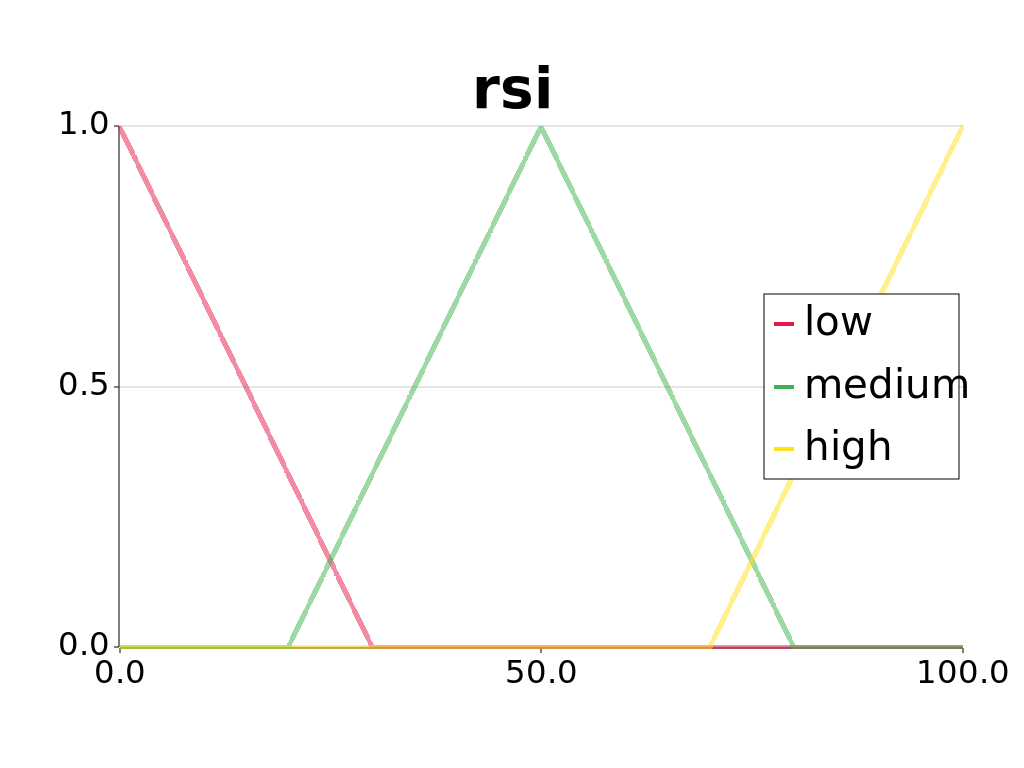
\includegraphics[width = \linewidth]{rsi.png}
    \end{subfigure}
    \begin{subfigure}{.45\textwidth}
        \centering
        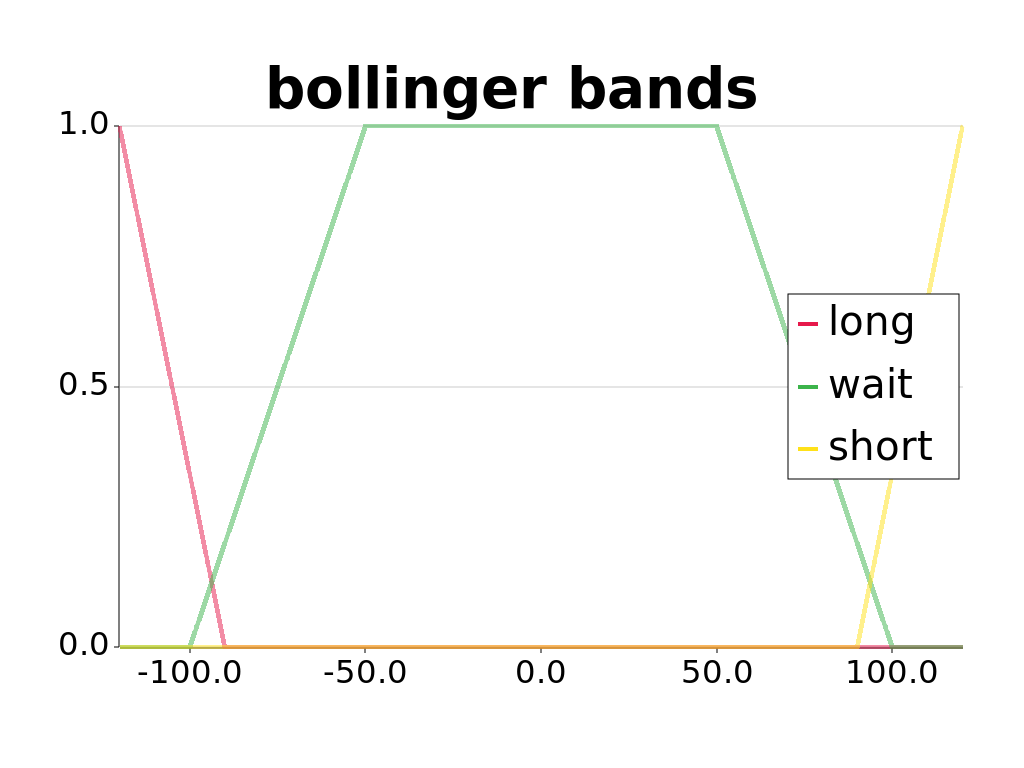
\includegraphics[width = \linewidth]{bb.png}
    \end{subfigure}
    \begin{subfigure}{\textwidth}
        \centering
        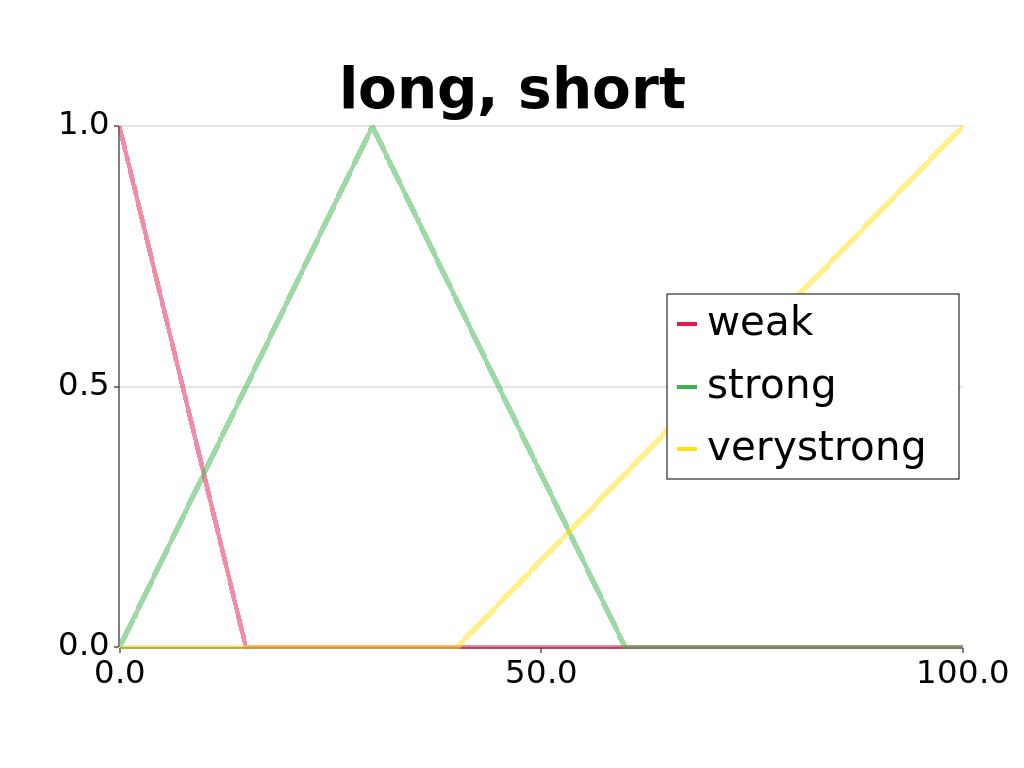
\includegraphics[width = 0.5\linewidth]{ls.png}
    \end{subfigure}

    \caption{Fuzzifications of the indicators and outputs}
    \label{fig:1}
\end{figure}
\FloatBarrier
Follwing the common interpretation of both RSI and Bollinger Bands, we create fuzzy rules to match with those interpretation 
as shown on \cref{table:3}.

\begin{table}[htp]
	\centering
	\begin{tabular}{c c c c}
		\toprule
        {RSI} & {Bollinger Bands} & {LONG} & {SHORT} \\ 
        \midrule
        HIGH & LONG & WEAK & WEAK \\
        HIGH & WAIT & WEAK & STRONG \\
        HIGH & SHORT & WEAK & VERYSTRONG \\
        MEDIUM & LONG & WEAK & STRONG \\
        MEDIUM & WAIT & WEAK & WEAK \\
        MEDIUM & SHORT & STRONG & WEAK \\
        LOW & LONG & VERYSTRONG & WEAK \\
        LOW & WAIT & STRONG & WEAK \\
        LOW & SHORT & WEAK & WEAK \\
        \bottomrule
    \end{tabular} 
    \caption{Fuzzy rules.}
	\label{table:3}
\end{table}
\FloatBarrier

\begin{figure}[ht]
    \centering
    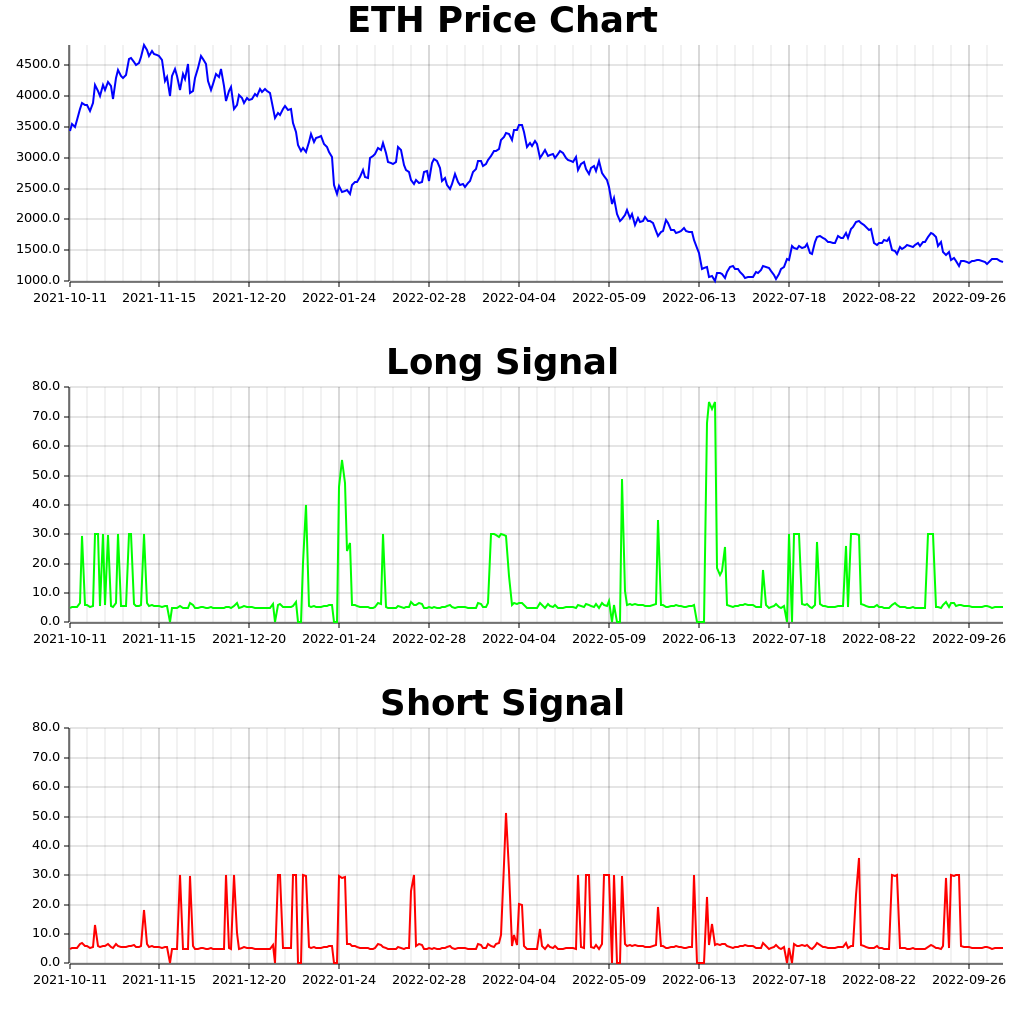
\includegraphics[scale=0.45]{chart.png}
    \caption{Result of fuzzy rules apply on each day from 2021-10-11 to 2022-10-09 where ETH price chart 
    is the price in USD (obtained from coingecko), long signal is a defuzzification result of output LONG, and short signal is a 
    defuzzification result of output SHORT.}
    \label{fig:2}
\end{figure}
\FloatBarrier

\section*{Experiment \& Analysis}
We get ETH price data from coingecko, and apply our fuzzy rules using RSI and Bollinger Bands as inputs as we described in \nameref{tech} on each
day from 2022-10-11 to 2022-10-09. The result can be seen on \cref{fig:2} which we can see the spikes on both long and short signal graph, 
those spikes is what we will be interest on as an entry point. Next, we set up backtesting 
(the general method for seeing how well a strategy or model would have done) for both classic and fuzzy rules with these rules:
\begin{enumerate}
    \item Initial capital is 1000\$ and we are not reinvesting any trade profit/loss into capital.
    \item {We iterate over all data from 2022-10-11 to 2022-10-09 and entry a position of 100\$ following these conditions: 
        \begin{itemize}
            \item For fuzzy rules, if either long or short signal is greater than 40 we enter that position.
            \item For classisc rule, we use the exact same rules as shown on \cref{table:1} and \cref{table:2}
        \end{itemize}
    }
    \item {For each position, we take profit if the price difference (profit side) is greater than 20\% 
        and stop-loss if the price difference (loss side) is greater than 10\%
    }
\end{enumerate}
The backtesting result is shown on \cref{table:4}, which we can see that if we combine both fuzzy long and short signals we get more
profit than both classic long and short signals combined. But, this might be from my poor design of classic rules examples however 
classic rules can't provide us with the signal graph that is intuitive like fuzzy rules (as shown on \cref{fig:2})
because the results of classic rules can be only 1 or 0. The fuzzy signal graph can visualize how likely you shoukd enter a market 
e.g. the big spike on long signal, we can consider entering a position with more confidence because of it (which is likely to make us 
a profit as we can see that the price is getting up considerably higher).

\begin{table}[htp]
	\centering
	\begin{tabular}{c c c c c c c}
		\toprule
        {Signal used} & {Total trade} & {Profit trade} & {Loss trade} & {Total profit (\$)} & {Total loss (\$)} & {Net profit (\$)} \\ 
        \midrule
        Fuzzy Long & 9 & 6 & 3 & 139.26 & -40.132 & 99.131 \\
        Fuzzy Short & 1 & 1 & 0 & 20.624 & 0.000 & 20.624 \\
        Classic Long & 10 & 5 & 5 & 111.541 & -85.499 & 26.043 \\
        Classic Short & 3 & 3 & 0 & 61.244 & 0.000 & 61.244 \\
        \bottomrule
    \end{tabular} 
    \caption{Backtesting result.}
	\label{table:4}
\end{table}
\FloatBarrier

\section*{Conclusion}
Fuzzy logic can be useful for trading securities because of its ability to deal with uncertainty and vagueness
we can use more than just for entry rules for example we can use it for exit rules, setting a position size,
etc. And the ability to visualize how fuzzy rules result in the signal graph can be a huge difference when
deciding to enter a market. Furthermore, we can add more linguistic variables which we tailor to our likes
or more rules to make fuzzy rules more practical and useful.


\newpage
\printbibliography

\subfile{appendix}

\end{document}